\documentclass{ximera} 

\input{../preamble}
\input{../preamblekdn}
\addPrintStyle{..}

\begin{document}
	\author{Koen De Naeghel - Wiskunde Op Maat}
	\xmtitle{Oefeningen reeks 3}{}
    \xmsource
	\label{xim:veeltermen_toepassingen_oefeningen_reeks3}
%%\section*{Oefeningen reeks 3}

\begin{exercise}
Bepaal alle kubische veeltermen \(A(x)\) waarvan de constante term gelijk is aan nul en waarvoor geldt dat
\[
A(x) - A(x-1) = x^2.
\]

% \(A(x) = \answer[onlineshowanswerbutton]{\frac{1}{3}\,x^3 + \frac{1}{2}\,x^2 + \frac{1}{6}\,x + d\( met \)d \in \R } \)
\begin{uitkomst}
$$
A(x) = \frac{1}{3}\,x^3 + \frac{1}{2}\,x^2 + \frac{1}{6}\,x + d \text{ met } d \in \R 
$$
\end{uitkomst}
\end{exercise}

\begin{Uitbreiding}
\begin{exercise}
In wiskunde staat een \underline{bewijs zonder woorden}\index{bewijs zonder woorden} voor een figuur die aangeeft dat een bepaalde wiskundige uitspraak vanzelfsprekend is, zonder dat daarbij begeleidende uitleg vermeld wordt. Daarbij gaat het vaak om identiteiten in de algebra of stellingen in de meetkunde. Zo werden al bewijzen zonder woorden gevonden van de stelling van Pythagoras, de cosinusregel en formules voor sommen van getallen die aan een bepaalde regelmaat voldoen, zoals de eindige som 
\[
1 + 2 + 3 + \dots + n 
\]
met \(n \in \N_0\) willekeurig, en de niet-eindigende sommen 
\[
0,9 + 0,09 + 0,009 + \dots \quad \text{ en } \quad 1 + \frac{1}{2} + \frac{1}{4} + \frac{1}{8} + \dots
\]
Een bewijs zonder woorden geldt niet als een volledig bewijs zoals we dat in wiskunde kennen, omdat de logische argumenten ontbreken om de uitspraak formeel aan te tonen. Het kan wel waardevolle intuïtieve ideëen aanreiken. Op die manier kan er voor elk bewijs zonder woorden een redenering worden opgeschreven die gebaseerd is op de figuur en die kan gelden als een volledig bewijs van de uitspraak. 

Hieronder staat een bewijs zonder woorden van een merkwaardig product. Formuleer de bijbehorende uitspraak en schrijf op basis van de figuur een volledig bewijs op.

% \medskip

% %%%%%%%%%%%%%%%%%%%%%%%%%%%%%%%%%%%%%%%%%%%%%%%%%%%%%%%%%%%%%%%%%%%%%%%%%
% \begin{center}
% \psset{xunit=0.75cm,yunit=0.75cm}
% \begin{pspicture}(2.5,0)(8,5.5) % co linksonder, co rechtsboven

% \psline[](3,0)(8,0)(8,5)(3,5)(3,0)

% \psline[](3,1)(8,1)
% \psline[](7,0)(7,5)

% \uput[u](7.5,0.2){\(b^2\)}
% \uput[u](5,0.2){\(ab\)}
% \uput[u](7.5,2.7){\(ab\)}
% \uput[u](5,2.7){\(a^2\)}

% \uput[u](2.7,2.7){\(a\)}
% \uput[u](2.7,0.2){\(b\)}

% \uput[u](5,5){\(a\)}
% \uput[u](7.5,5){\(b\)}
% \end{pspicture}
% \end{center}
%%%%%%%%%%%%%%%%%%%%%%%%%%%%%%%%%%%%%%%%%%%%%%%%%%%%%%%%%%%%%%%%%%%%%%%%%
\begin{image}[\width]
	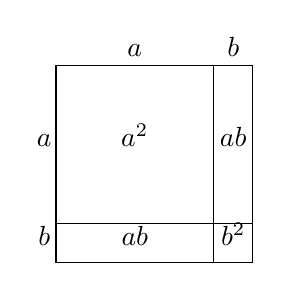
\begin{tikzpicture}[x=0.5cm, y=0.5cm]

		% Outer rectangle
		\draw (3,0) rectangle (8,5);
		
		% Horizontal division at y=1
		\draw (3,1) -- (8,1);
		
		% Vertical division at x=7
		\draw (7,0) -- (7,5);
		
		% Labels for the areas
		\node[above] at (7.5,0.2) {\(b^2\)};
		\node[above] at (5,0.2) {\(ab\)};
		\node[above] at (7.5,2.7) {\(ab\)};
		\node[above] at (5,2.7) {\(a^2\)};
		
		% Labels for dimensions on the left side
		\node[above] at (2.7,2.7) {\(a\)};
		\node[above] at (2.7,0.2) {\(b\)};
		
		% Labels on the top
		\node[above] at (5,5) {\(a\)};
		\node[above] at (7.5,5) {\(b\)};
		
	\end{tikzpicture}
\end{image}


\begin{uitkomst}
Deze figuur toont waarom voor elke \(a,b \in \R^+_0\) geldt dat \((a+b)^2 = a^2 + 2ab + b^2\).

Inderdaad, want het grote vierkant heeft zijde \(a+b\), en dus oppervlakte \((a+b)^2\). 
En het bestaat uit twee kleinere vierkanten met oppervlaktes respectievelijk \(a^2\) en \(b^2\), en twee keer een rechthoek met oppervalkte \(ab\).
De totale oppervlakte is dus \(a^2+b^2+2ab\)
\\
Dit bewijst de gelijkheid \((a+b)^2 = a^2 + 2ab + b^2\)
\end{uitkomst}

\end{exercise}
\end{Uitbreiding}

%%% \clearpage

\begin{exercise}
Ontbind telkens de veelterm zo ver mogelijk in factoren. Ga algebraïsch te werk en schrijf jouw redenering uit.  

	\begin{question} \(x^4+1\)         \begin{uitkomst} \((x^2+\sqrt{2}\,x+1)(x^2-\sqrt{2}\,x+1)                                                    \) \end{uitkomst} \end{question}
	\begin{question} \(x^4 + x^2 + 1\) \begin{uitkomst} \((x^2+x+1)(x^2-x+1)                                                                        \) \end{uitkomst} \end{question}
	\begin{question} \(x^5-1\)         \begin{uitkomst} \((x-1)\left(x^2+\frac{1+\sqrt{5}}{2}\,x+1\right)\left(x^2+\frac{1-\sqrt{5}}{2}\,x+1\right) \) \end{uitkomst} \end{question}
	\begin{question} \(x^5+1\)         \begin{uitkomst} \((x-1)\left(x^2-\frac{1+\sqrt{5}}{2}\,x+1\right)\left(x^2-\frac{1-\sqrt{5}}{2}\,x+1\right) \) \end{uitkomst} \end{question}
\end{exercise}

	

\begin{exercise}
Zij \(A(x)\) een willekeurige veelterm met gehele coëfficiënten en met hoogstegraadscoëfficiënt gelijk aan \(1\). Toon aan: als \(A(x)\) een rationale nulwaarde heeft, dan heeft \(A(x)\) ook een gehele nulwaarde.
\end{exercise}

\begin{Uitbreiding}
\begin{exercise}
Toon telkens de veeltermgelijkheid aan. Hierbij is \(a\) een willekeurig reëel getal en \(n \in \N_0\).

\begin{question}
	\(\D x^{n+1} - a^{n+1} = (x-a)(x^{n} + ax^{n-1} + a^2x^{n-2} + \dots + a^{n-2}x^2 + a^{n-1}x + a^{n})\)
\end{question}
\begin{question}
	\(\D x^{2n+1} + a^{2n+1} = (x+a)(x^{2n} - ax^{2n-1} + a^2x^{2n-2} - a^3x^{2n-3} + \dots - a^{2n-1}x + a^{2n})\)
\end{question}
\end{exercise}

\begin{exercise}
\label{somtweevierdemachten}
Toon voor elke \(a \in \R_0\) aan dat het zo ver mogelijk ontbinden in factoren van de veeltermen \(x^2 \pm a^2\), \(x^3 \pm a^3\), \(x^4 \pm a^4\) en  \(x^5 \pm a^5\) wordt gegeven door onderstaande uitdrukkingen. Hierbij staat \(\varphi\) voor de gulden snede. %{\wsgref{gulden snede}{Bijzondere irrationale getallen}{22}}. 
\begin{align*}
& x^2 + a^2 = x^2 + a^2 && \text{som van twee kwadraten} \\
& x^2 - a^2 = (x-a)(x+a) && \text{verschil van twee kwadraten} \\
& x^3 + a^3 = (x+a)(x^2 - ax + a^2) && \text{som van twee derde machten} \\
& x^3 - a^3 = (x-a)(x^2 + ax + a^2) && \text{verschil van twee derde machten} \\
& x^4 + a^4 = (x^2 + \sqrt{2}\,ax + a^2)(x^2 - \sqrt{2}\,ax + a^2) && \text{som van twee vierde machten} \\
& x^4 - a^4 = (x-a)(x+a)(x^2+a^2) && \text{verschil van twee vierde machten} \\
& x^5 + a^5 = (x+a)(x^2-\varphi\,ax + a^2)(x^2+\frac{1}{\varphi}\,ax + a^2) && \text{som van twee vijfde machten} \\
& x^5 - a^5 = (x-a)(x^2+\varphi\,ax + a^2)(x^2-\frac{1}{\varphi}\,ax + a^2) && \text{verschil van twee vijfde machten}
\end{align*}
\end{exercise}

\begin{exercise}
{\bf (gehele wortelstelling)}\index{gehele wortelstelling} 
In deze oefening bewijzen we de gehelewortelstelling: 
\begin{itemize}
\item[]
Zij \(A(x)\) een veelterm met gehele coëfficiënten. Als \(a \neq 0\) een gehele nulwaarde van \(A(x)\) is, dan is \(a\) een deler van de constante term.
\end{itemize}
Beschouw een willekeurige veelterm met gehele coëfficiënten:
\[
A(x) = a_0 + a_1 x + a_2 x^2 + \dots + a_{n-1} x^{n-1} + a_nx^n
\]
waarbij \( n \in \N\) en \(a_0, a_1, \ldots, a_n \in \Z\). Stel nu dat \(a \neq 0\) een gehele nulwaarde van deze veelterm is, dus
\[
a \in \Z_0 \quad \text{ en } \quad A(a) = 0.
\]
Toon aan dat \(A(a) = 0\) leidt tot \(a_0 = a\cdot q\) voor een zeker geheel getal \(q\), en dus dat \(a \mid a_0\). 
\end{exercise}
\end{Uitbreiding}

%%% \clearpage

\begin{Uitbreiding}
\begin{exercise}\label{oefening:rationalewortelstelling}
{\bf (rationale wortelstelling)}\index{rationale wortelstelling} 
In deze oefening bewijzen we de rationale wortelstelling:
\begin{itemize}
\item[]
Zij \(A(x)\) een veelterm met gehele coëfficiënten. Als \(\frac{p}{q} \neq 0\) een rationale nulwaarde van \(A(x)\) is (met \(p,q\) gehele getallen en \(\frac{p}{q}\) onvereenvoudigbaar), dan is \(p\) een deler van de constante term en \(q\) een deler van de hoogstegraadscoëfficiënt  
\end{itemize}
Beschouw een willekeurige veelterm met gehele coëfficiënten:
Beschouw een willekeurige veelterm met gehele coëfficiënten:
\[
A(x) = a_0 + a_1 x + a_2 x^2 + \dots + a_{n-1} x^{n-1} + a_nx^n
\]
waarbij \( n \in \N\) en \(a_0, a_1, \ldots, a_n \in \Z\). Beschouw nu een rationaal getal \(\frac{p}{q} \neq 0\), en stel dat dit getal een nulwaarde van deze veelterm is waarbij \(p,q\) gehele getallen en \(\frac{p}{q}\) onvereenvoudigbaar, dus
\[
p,q \in \Z_0 \quad \text{ en } \quad \ggd(p,q)=1 \quad \text{ en } \quad A\left(\frac{p}{q}\right) = 0.
\]
Toon aan dat \(A\left(\frac{p}{q}\right) = 0\) leidt tot \(p \mid a_0q^n\) en \(q \mid a_n p^n\), en dus tot \(p \mid a_0\) en \(q \mid a_n\).
\end{exercise}
\end{Uitbreiding}

\begin{exercise}
Bepaal algebraïsch alle reële getallen \(x\) waarvoor geldt dat 
\[
x^3-288x^2-282x  = 2023.
\]
Schrijf alle tussenstappen op.
Antwoord: \( x = \answer[onlineshowanswerbutton]{289}\)
\end{exercise}

\begin{exercise}
Bepaal algebraïsch alle nulwaarden van de veelterm
\[
A(x) = x^6 + x^4 + x^2 + 1.
\]
Schrijf alle tussenstappen op.
Antwoord: \(x = \answer[onlinenoinput]{ \text{ (er zijn geen reële nulwaarden)}}\)
\end{exercise}

\begin{exercise}
Bepaal een veelterm met gehele coëfficiënten waarvan \(\sqrt{3+\sqrt{17}}\) een nulwaarde is.

Antwoord: \(A(x) = \answer[onlineshowanswerbutton]{x^4-6x^2-8}\)
\end{exercise}

\begin{Uitbreiding}
\begin{exercise}
In deze oefening laten we zien dat de rationale wortelstelling gebruikt kan worden om aan te tonen dat sommige reëele getallen irrationaal zijn.
\begin{enumerate}

\item
Bepaal een veelterm \(A(x)\) met gehele coëfficiënten waarvan \(\sqrt{2}\) een nulwaarde is.
\item
Toon met behulp van de rationale wortelstelling aan dat die veelterm \(A(x)\) geen rationale nulwaarden heeft.
\item
Argumenteer nu hoe uit (a) en (b) volgt dat \(\sqrt{2}\) een irrationaal getal is.
\item
Toon op een gelijkaardige manier aan dat de volgende reële getallen irrationaal zijn:
\[
\sqrt{17}, \qquad \sqrt[3]{2}, \qquad \sqrt[7]{13} \qquad \sqrt{3+\sqrt{17}}, 
\qquad \text{ en } \qquad \sqrt{2}+\sqrt{3}.
\]
\end{enumerate}
\end{exercise}
\end{Uitbreiding}

\end{document}